\section{Parity}
%% Much of this is taken from
%% Sakurai
We consider now the discrete transformation of space inversion, or \emph{parity}.
Firstly, basic properties of the transformation will be presented and discussed.
Its effect on the position, momentum, and angular momentum operators will be discussed, before a more general discussion on how it transforms proper- and pseudo-tensors.
This will be applied to see how the parity transformation affects electric and magnetic fields.

Let the parity operator $P$ be a unitary operator
\begin{equation}
  P: \quad \ket{a} \rightarrow P\ket{a}.
\end{equation}
By definition, we require
\begin{align}
  P^\dagger x P &= -x,\\
  P^\dagger p P &= -p,
\end{align}
where $x, p$ are the position and momentum operators.
By the unitarity of $P$, which means that $P^\dagger P = I$,
$$
xP = -Px.
$$
We now use this anticommutation to find an explicit form of the transformation in the position representation.
By noting that, given the position eigenstate $\ket{x_1}$,
\begin{equation}
  x P\ket{x_1} = -P x_1\ket{x_1} = -x_1 P\ket{x_1},
\end{equation}
with $x_1$ the eigenvalue of the state, we may conclude
$$
P\ket{x_1} = \ket{-x_1}
$$
up to some arbitrary phase.
We chose this phase to be unity.
Then
\begin{equation}
  P^2 \ket{x_1} = \ket{x_1}
\end{equation}
for any position eigenstate, which  gives the  operator relation $P^2 = 1 \implies P = \pm 1$.
This also means that $P$ is Hermitian,
$$
P = P^{-1} = P^\dagger.
$$

The treatment of angular momentum is somewhat more involved.
Some sources simply state that as the orbital angular momentum
$$
L = x \times p
$$
is a product of two odd quantities, it must be even under parity.
This, of course, is a gross over simplification, as extra care must be taken when considering the spin angular momentum $S$ contributing to the total angular momentum
$$
J = L + S.
$$
The angular momentum operator is the generator of rotations
$$
R = e^{-i \epsilon J\cdot n} \approx 1 - i \epsilon J \cdot n
$$
where we expanded the operator under the assumption of a small angle, $\epsilon \ll 1$.
As rotations are invariant during space inversion,
\begin{align}
  P^\dagger R P &= R\\
 \mathllap{\implies\;} P^\dagger J \cdot n P &= J\cdot n
\end{align}
from which it follows that
\begin{equation}
P^\dagger J P = J,
\end{equation}
as the parity operator obviously does not act on the normal vector $n$.
Thus, the angular momentum operator, unlike the linear momentum operator, is even under parity.

For a general vector-like\footnote{We use the term \emph{vector-like} instead of vector, as the term vector is defined as something that is odd under parity, as opposed to for example a pseudo vector, even though they naively ``look'' like vectors. This can be compared to tensors. The definition of a tensor is something that transforms like a tensor under a Lorentz transformation, so we may have matrix objects that ``look'' like tensors, but transforms differently.} quantity $V$, we will consider how it transforms during space inversion.
If the quantity ``flips'' during space inversion, $P^\dagger V P = -V$, we say simply that it is a vector, also sometimes known as a polar vector.
Quantities that do not ``flip'', so that they turn into their opposites in the flipped image, we denote pseudo vectors.
Thus, depending on whether the eigenvalue of an operator under space inversion is $+1$ or $-1$ we say that it is either a pseudo-vector or vector, respectively.
Position and momentum are examples of vectors, while angular momentum and the magnetic field are examples of pseudo-vectors.
An illustrative explanation of this is shown in \cref{fig:pseudovector}, which explains both angular momentum and magnetic fields.

\emph{Remark about dimensionality}: The above discussion about parity, which is the standard way to present parity in condensed matter physics, is valid for three dimensions.
In two dimensions, however, one must separate \emph{parity} and \emph{space inversion}.
The former takes a right-handed system to a left-handed system~\cite{sakuraiModernQuantumMechanics2017}, while the latter inverts space, $\vec{x} \to  -\vec{x}$.
In odd dimensions this is the same, while in even dimensions they differ.
In even dimensions, inversion corresponds to a rotation, while a parity transform is different from any rotation.
In more formal terms, inversion is part of the group of proper  rotations $SO(n)$ for even dimensions, as the determinant is $+1$, the definition of a proper rotation.
Parity should in general be taken to be the operation $P$ such that the group of all rotations $O(n) = SO(n) \times \{E, P\}$, with $E$ the identity transformation.
This will not be of direct importance here, but it is an important detail to note.

\begin{figure}[h]
  \centering
  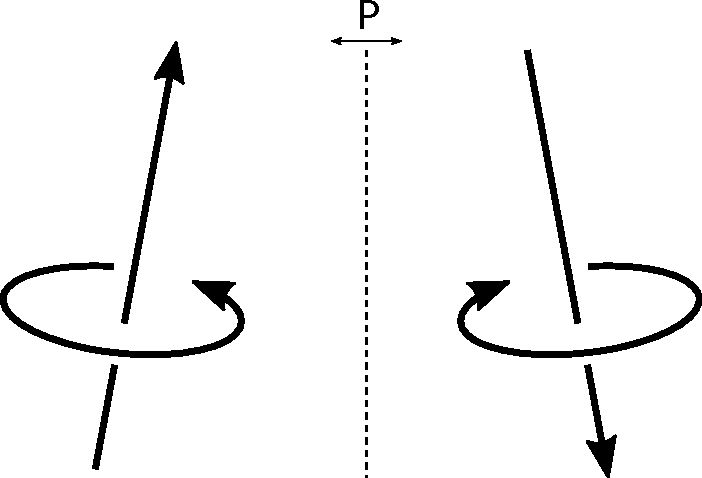
\includegraphics[width=0.5\textwidth]{figures/pseudovector}
  \caption{Schematic illustration of vectors and pseudovectors.
    A vector field with curl, which may be taken to be either momentum or current, is shown as a rotating arrow.
    The curl of this field, which will respectively be the angular  momentum or $B$-field, is shown as a straight arrow.
    Under inversion, shown as a mirror operation, the curl generated by the field is inverted in addition to the mirroring, i.e. rotated.
    This non-formal illustration gives an intuitive explanation of the concepts vector and pseudovector.
    Note that as the example is two-dimensional, mirror symmetry here the same as parity, and not inversion.
    See main text for details.
  }
  \label{fig:pseudovector}
\end{figure}
